% Compile with: pdflatex language-orchestration-research-spec.tex
\documentclass[11pt]{article}

\usepackage[margin=1in]{geometry}
\usepackage[T1]{fontenc}
\usepackage[utf8]{inputenc}
\usepackage{lmodern}
\usepackage{microtype}
\usepackage{amsmath,amssymb}
\usepackage{booktabs}
\usepackage{tabularx}
\usepackage{xcolor}
\usepackage{hyperref}
\usepackage[nameinlink,noabbrev]{cleveref}
\usepackage[section]{placeins}
\usepackage{tikz}
\usetikzlibrary{arrows.meta,positioning,calc,fit,shapes.geometric,shapes.misc}

\hypersetup{
  colorlinks=true,
  linkcolor=blue!50!black,
  citecolor=blue!50!black,
  urlcolor=blue!60!black,
  pdftitle={CoTCodec: Language Choice as an Orchestration Variable for Tool-Using LLM Agents},
  pdfauthor={Kevin Liu}
}

\definecolor{specblue}{HTML}{2E5AAC}
\definecolor{specred}{HTML}{B44A4A}
\definecolor{specgold}{HTML}{B67814}
\definecolor{specgreen}{HTML}{2F7D49}
\definecolor{specgray}{HTML}{59636E}

\tikzset{
  box/.style={draw, rounded corners=4pt, thick, align=center, fill=blue!6, text width=2.8cm, minimum height=1cm},
  widebox/.style={draw, rounded corners=4pt, thick, align=center, fill=blue!6, text width=3.7cm, minimum height=1cm},
  fixedbox/.style={draw, rounded corners=4pt, thick, align=center, fill=gray!14, text width=2.6cm, minimum height=1cm},
  mixedbox/.style={draw, rounded corners=4pt, thick, align=center, fill=orange!18, text width=2.8cm, minimum height=1cm},
  decision/.style={draw, diamond, aspect=2.2, thick, align=center, fill=yellow!15, text width=2.8cm, inner sep=1.5pt},
  line/.style={-Latex, thick}
}

\setlength{\parindent}{0pt}
\setlength{\parskip}{0.65em}

\title{\vspace{-1.5em}\textbf{CoTCodec: Language Choice as an Orchestration Variable for Tool-Using LLM Agents}\\[0.35em]\large A (Regretfully) Verbose Research Spec}
\author{Kevin Liu\\Princeton University}
\date{April 2026}

\begin{document}
\maketitle

\begin{abstract}
This mini-spec proposes an empirical study of language choice as an internal orchestration variable for tool-using large language model agents. The motivating observation is quite straightforward: equivalent content can occupy very different token budgets across languages, and recent reasoning-model work suggests that exposed chains of thought sometimes mix languages in ways that are not obviously accidental. The strongest recent evidence goes further: DeepSeek-R1 reports that reinforcement-learning post-training produced mixed-language reasoning traces and later introduced a language-consistency reward to suppress them. Li et al.\ argue that reinforcement learning with verifiable rewards is the key stage that induces language mixing in bilingual reasoning, while EfficientXLang reports 20--40\% token savings from cross-lingual reasoning without loss of accuracy. Taken together, these results suggest a systems question that has not yet been answered cleanly: can internal language routing improve the cost-latency-success frontier of realistic agent trajectories once tool overhead, retries, memory updates, and safety risks are all included?

The proposed intervention is deliberately narrow. User-facing responses, tool schemas, and structured arguments remain in English. Only framework-visible intermediate messages are allowed to vary: planner notes, subtask handoffs, memory summaries, retry diagnoses, and coordinator messages. The core hypothesis is that these messages behave like communication payloads, so language can function as a controllable compression protocol. The counter-hypothesis is equally important: fixed tool overhead, translation costs, schema drift, semantic drift on terminology-heavy reasoning, or multilingual safety failures may erase the gains. The specification therefore centers on paired evaluations across agent benchmarks, strong compression baselines, structured-reasoning baselines, semantic-fidelity checks, and multilingual safety checks. Recent work on abstract chain-of-thought further sharpens the positioning: language routing is the most practical inference-time-only intervention, while more aggressive non-verbal reasoning media raise a separate monitorability tradeoff that this broader research program will study later \cite{ramji2026abstractcot,baker2025monitoring,metr2025cotinformative}.
\end{abstract}

\section{Motivation}

The motivating anecdote for this project is operational rather than philosophical. In a 1v1 token count comparison for Anthropic models, text written in Polish translated to roughly 60\% more tokens than its English counterpart, meaning that Polish was materially more expensive and likely slower under that tokenizer. The same content rose from 36{,}637 tokens in English to 59{,}442 in Polish using an Anthropic-style tokenizer, a difference of 22{,}805 tokens or 62.25\%. On its own, however, that example would be too easy to overread. A single tokenizer anecdote cannot tell us whether non-English is generally cheaper, generally more expensive, or simply more variable.

\begin{figure}[t]
\centering
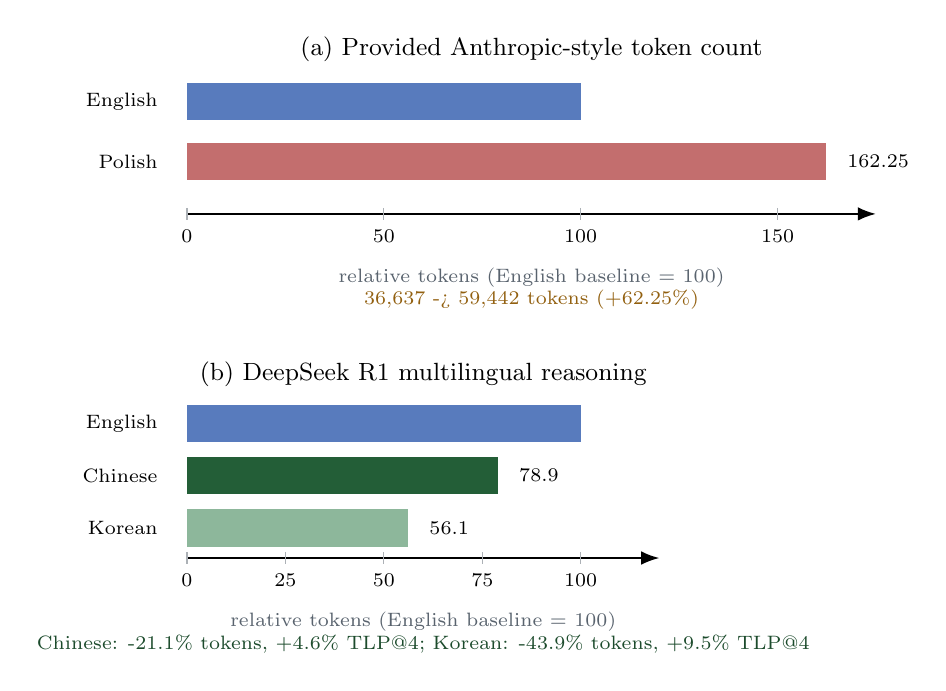
\begin{tikzpicture}[x=0.05cm,y=0.95cm]
  % Top panel
  \begin{scope}[shift={(0,4.6)}]
    \node[font=\small] at (87.5,2.2) {(a) Provided Anthropic-style token count};
    \fill[specblue!80] (0,1.25) rectangle (100,1.75);
    \fill[specred!80] (0,0.45) rectangle (162.25,0.95);
    \node[anchor=east, font=\scriptsize] at (-5,1.5) {English};
    \node[anchor=east, font=\scriptsize] at (-5,0.7) {Polish};
    \node[anchor=west, font=\scriptsize] at (165.25,0.7) {162.25};
    \draw[line] (0,0) -- (175,0);
    \foreach \x/\label in {0/0,50/50,100/100,150/150} {
      \draw[specgray!50] (\x,0.08) -- (\x,-0.08);
      \node[below, font=\scriptsize] at (\x,-0.08) {\label};
    }
    \node[font=\scriptsize, text=specgray] at (87.5,-0.85) {relative tokens (English baseline = 100)};
    \node[font=\scriptsize, text=specgold!80!black] at (87.5,-1.15) {36{,}637 -> 59{,}442 tokens (+62.25\%)};
  \end{scope}

  % Bottom panel
  \begin{scope}[shift={(0,0)}]
    \node[font=\small] at (60,2.45) {(b) DeepSeek R1 multilingual reasoning};
    \fill[specblue!80] (0,1.55) rectangle (100,2.05);
    \fill[specgreen!75!black] (0,0.85) rectangle (78.9,1.35);
    \fill[specgreen!55] (0,0.15) rectangle (56.1,0.65);
    \node[anchor=east, font=\scriptsize] at (-5,1.8) {English};
    \node[anchor=east, font=\scriptsize] at (-5,1.1) {Chinese};
    \node[anchor=east, font=\scriptsize] at (-5,0.4) {Korean};
    \node[anchor=west, font=\scriptsize] at (81.9,1.1) {78.9};
    \node[anchor=west, font=\scriptsize] at (59.1,0.4) {56.1};
    \draw[line] (0,0) -- (120,0);
    \foreach \x/\label in {0/0,25/25,50/50,75/75,100/100} {
      \draw[specgray!50] (\x,0.08) -- (\x,-0.08);
      \node[below, font=\scriptsize] at (\x,-0.08) {\label};
    }
    \node[font=\scriptsize, text=specgray] at (60,-0.85) {relative tokens (English baseline = 100)};
    \node[font=\scriptsize, text=specgreen!60!black, align=center] at (60,-1.15) {Chinese: -21.1\% tokens, +4.6\% TLP@4; Korean: -43.9\% tokens, +9.5\% TLP@4};
  \end{scope}
\end{tikzpicture}
\caption{Two motivating contrasts. Top: a provided Anthropic-style count where Polish inflates token usage relative to English. Bottom: cited multilingual reasoning results from DeepSeek R1, where Chinese and Korean use fewer tokens than English while preserving or improving task performance \cite{ahuja2025efficientxlang}. The point is not that non-English is uniformly cheaper or uniformly costlier. Cross-language efficiency is tokenizer-, model-, and task-dependent.}
\label{fig:token-gap}
\end{figure}

Figure~\ref{fig:token-gap} therefore makes a narrower and more defensible point than a slogan like ``non-English is cheaper.'' The broader literature often describes tokenization inequity as a token tax borne by many languages relative to English, and that framing is justified in aggregate \cite{petrov2023unfairness}. But the paired examples here show that the phenomenon is not absolute. Some languages are penalized under a particular tokenizer, while others can become more efficient internal reasoning media in a different model and task setup. Recent multilingual tokenization work gives that claim firmer footing. Petrov et al.\ show that translated equivalents can differ by up to 15$\times$ in tokenized length across languages \cite{petrov2023unfairness}. Limisiewicz et al.\ show that vocabulary allocation and overlap materially affect multilingual language modeling \cite{limisiewicz2023tokenization}. Rust et al.\ argue that tokenizer choice is not a negligible implementation detail for multilingual LLMs \cite{rust2023tokenizer}. Einarsson et al.\ then connect fragmentation to runtime directly, reporting roughly 3.4$\times$ fertility and 16.5$\times$ inference slowdown in a high-fragmentation orthography condition \cite{einarsson2026scripttax}. The implication is simple: if agent systems spend a large share of their budget on internally generated text, then internal representation choice deserves the same attention we already give to tool selection, memory compression, and retrieval policy.

\section{Why This Question Is Now Empirically Viable}

Until recently, the idea that models might switch languages strategically during reasoning would have sounded like a prompt-engineering curiosity. The evidence is now much stronger. Reasoning-focused models have begun to expose mixed-language traces in ways that are systematic enough to study, and the relevant papers no longer live at the level of anecdote.

\begin{figure}[t]
\centering
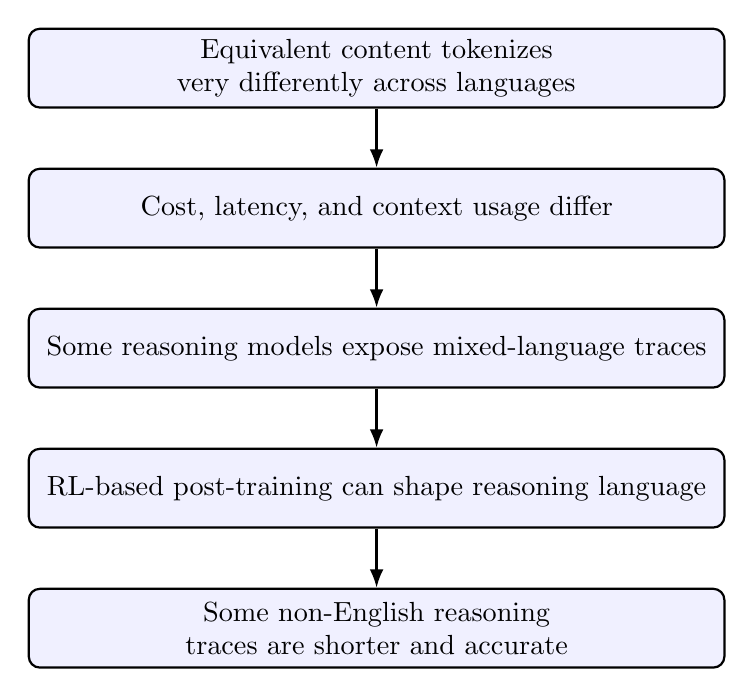
\begin{tikzpicture}[node distance=0.75cm]
  \node[widebox, text width=8.6cm] (a) {Equivalent content tokenizes very differently across languages};
  \node[widebox, text width=8.6cm, below=of a] (b) {Cost, latency, and context usage differ};
  \node[widebox, text width=8.6cm, below=of b] (c) {Some reasoning models expose mixed-language traces};
  \node[widebox, text width=8.6cm, below=of c] (d) {RL-based post-training can shape reasoning language};
  \node[widebox, text width=8.6cm, below=of d] (e) {Some non-English reasoning traces are shorter and accurate};
  \draw[line] (a) -- (b);
  \draw[line] (b) -- (c);
  \draw[line] (c) -- (d);
  \draw[line] (d) -- (e);
\end{tikzpicture}
\caption{Evidence ladder. The proposed project sits on top of several empirical results that now exist in the literature but have not yet been unified at the agent-systems layer.}
\label{fig:evidence-ladder}
\end{figure}

DeepSeek-R1 is the most important starting point. The Nature version reports that DeepSeek-R1-Zero sometimes mixed English and Chinese during exposed chains of thought, and that a language-consistency reward was later introduced during reinforcement learning to suppress the behavior for readability reasons \cite{deepseek2025nature}. The paper notes that this intervention caused a slight performance degradation. That is exactly the kind of detail that turns a curiosity into a real scientific clue: reasoning-language behavior appears to have been entangled with whatever policy the model found reward-maximizing.

Li et al.\ sharpen that clue substantially. In \emph{The Impact of Language Mixing on Bilingual LLM Reasoning}, they argue that reinforcement learning with verifiable rewards is the critical stage that induces language mixing in bilingual reasoning models \cite{li2025bilingual}. They report that forcing monolingual decoding reduces accuracy by 5.6 points on MATH500, while a lightweight probe-guided switching intervention improves it by 2.92 points. Wang et al.\ broaden the picture, showing that language mixing in reasoning models is systematic across 15 languages, 18 subject areas, and multiple difficulty levels, and that script composition in reasoning traces aligns with internal representations \cite{wang2025mixing}. These papers do not prove that token efficiency is the sole cause of language switching, but they do establish that reasoning language is part of the learned policy rather than harmless surface noise.

EfficientXLang then supplies the missing efficiency result. Ahuja et al.\ report 20--40\% token savings from cross-lingual reasoning without accuracy loss and, in several cases, with accuracy gains \cite{ahuja2025efficientxlang}. Their DeepSeek R1 results are especially provocative: Chinese yields 21.1\% fewer tokens with a 4.6\% improvement in TLP@4, Russian yields 14.1\% fewer tokens with a 4.3\% improvement, and Korean yields 43.9\% fewer tokens with a 9.5\% improvement. They also translate non-English reasoning traces back into English and show that they often remain shorter than native English traces, suggesting that the effect is not reducible to script compression alone. This is the strongest current evidence that language choice can alter reasoning trajectories, not just the string length of a fixed trajectory.

A second recent result changes how to position this paper. Ramji et al.\ show that abstract chain-of-thought can compress reasoning by an order of magnitude using a learned discrete codebook rather than any human language \cite{ramji2026abstractcot}. That result does not obsolete language routing. It sharpens the boundary. Language routing is an inference-time intervention that requires no retraining; abstract chain-of-thought is a post-training intervention that may be much more efficient but also raises monitorability questions that matter for safety \cite{baker2025monitoring,metr2025cotinformative}. The clean claim for this paper is therefore narrower and stronger: among interventions a practitioner can apply at inference time to a fixed tool-using model, internal language routing is one of the most tractable candidates.

Two mechanism hypotheses should be kept separate. The first is tokenizer and representation efficiency: some languages simply consume fewer tokens under a given tokenizer, which increases the amount of working state the agent can preserve inside a fixed context window. The second is English-centric latent reasoning. Schut et al.\ argue that multilingual LLMs make key decisions in a representation space closest to English regardless of the surface input or output language \cite{schut2025english}, while Tam et al.\ find that large reasoning models tend to default to high-resource languages such as English at test time \cite{tam2025languagematters}. Qi et al.\ further show that forcing models to reason in the user's language improves readability and oversight but often lowers accuracy \cite{qi2025yourlanguage}. The present project cannot fully disentangle these mechanisms, but it can test whether the systems benefit of language routing looks more like pure token savings, a shift in reasoning trajectory, or some mixture of the two.

\section{Agents As A Paradigm}

The project is easier to motivate if ``agent'' is defined concretely. In this spec, an agent is an LLM-centered system that repeatedly reasons over the current state, chooses an action or tool call, observes the result, updates working memory, and decides what to do next. This closed-loop view matches the framing of recent surveys on LLM-based autonomous agents \cite{wang2023surveyagents}. It also matches the main line of influential systems papers. ReAct interleaves reasoning and acting \cite{yao2023react}. Toolformer shows that models can learn when and how to invoke tools \cite{schick2023toolformer}. AutoGen treats multi-agent conversation as a workflow primitive rather than a prompt-engineering trick \cite{wu2023autogen}. LLMCompiler explicitly treats function-call orchestration as a planning and scheduling problem \cite{kim2023llmcompiler}.

The reason agents have become a paradigm, rather than just a convenient wrapper around prompting, is that many valuable tasks are not solvable in one forward pass. Web interaction, retrieval, scheduling, code repair, customer support, and enterprise workflows all require iterative stateful behavior. The system has to decide what to inspect, what to call, what to remember, and when to stop. That shift from one-shot completion to closed-loop control is precisely what makes internal communication important.

\begin{figure}[t]
\centering
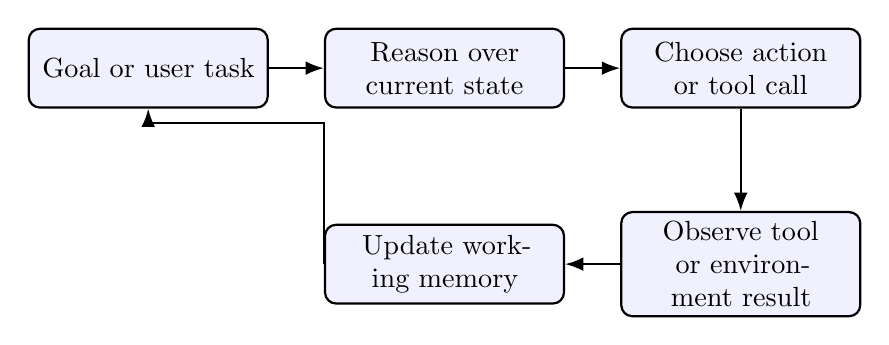
\begin{tikzpicture}[node distance=0.8cm and 0.7cm]
  \node[widebox, text width=2.8cm] (goal) {Goal or user task};
  \node[widebox, text width=2.8cm, right=of goal] (reason) {Reason over current state};
  \node[widebox, text width=2.8cm, right=of reason] (act) {Choose action or tool call};
  \node[widebox, text width=2.8cm, below=1.3cm of act] (obs) {Observe tool or environment result};
  \node[widebox, text width=2.8cm, left=of obs] (mem) {Update working memory};
  \draw[line] (goal) -- (reason);
  \draw[line] (reason) -- (act);
  \draw[line] (act) -- (obs);
  \draw[line] (obs) -- (mem);
  \draw[line] (mem.west) |- ($(goal.south)+(0,-0.18)$) -- (goal.south);
\end{tikzpicture}
\caption{Minimal agent loop. Agents differ from one-shot prompting because they repeatedly reason, act, observe, and update internal state.}
\label{fig:agent-loop}
\end{figure}

Once that loop exists, orchestration becomes a first-class design problem. A system is no longer only generating an answer. It is coordinating reasoning, tools, memory, and recovery from error. That is why language choice becomes interesting at the systems layer. Internal text is no longer just prose; it is one of the media through which the agent coordinates itself.

\section{Core Thesis}

The present spec takes the following position: internal language choice should be studied as an orchestration policy over explicit agent messages, not as a claim about hidden cognition and not as a blanket statement that one language ``thinks better'' than another. The intervention is narrow on purpose. User-visible responses remain English. Tool schemas, function names, JSON keys, and structured arguments remain English. Only framework-visible intermediate messages are permitted to vary.

Those messages include planner notes, subtask briefs, coordination messages, memory summaries, retry diagnoses, and other pieces of text that agent frameworks already externalize. In other words, the target is communication, not ontology. This distinction is important because it keeps the project reproducible and avoids making claims about inaccessible provider-private chain-of-thought.

\begin{figure}[t]
\centering
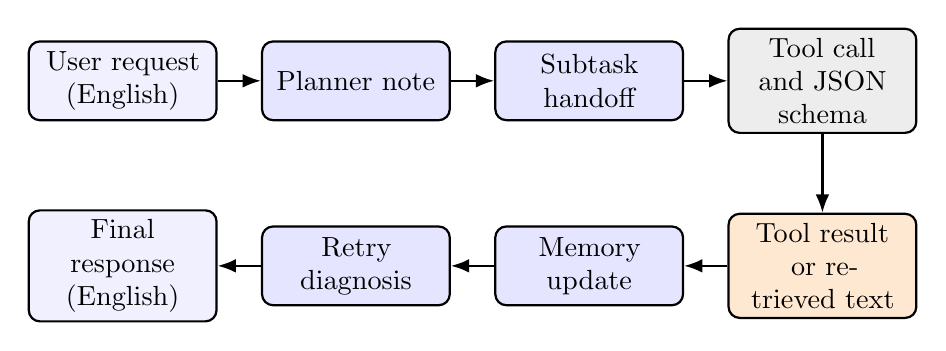
\begin{tikzpicture}[node distance=0.55cm and 0.55cm]
  \node[box, text width=2.15cm] (u) {User request\\(English)};
  \node[box, text width=2.15cm, right=of u, fill=blue!10] (p) {Planner note};
  \node[box, text width=2.15cm, right=of p, fill=blue!10] (h) {Subtask handoff};
  \node[fixedbox, text width=2.15cm, right=of h] (t) {Tool call\\and JSON schema};
  \node[mixedbox, text width=2.15cm, below=1.0cm of t] (r) {Tool result\\or retrieved text};
  \node[box, text width=2.15cm, left=of r, fill=blue!10] (m) {Memory update};
  \node[box, text width=2.15cm, left=of m, fill=blue!10] (d) {Retry diagnosis};
  \node[box, text width=2.15cm, left=of d] (o) {Final response\\(English)};
  \draw[line] (u) -- (p);
  \draw[line] (p) -- (h);
  \draw[line] (h) -- (t);
  \draw[line] (t) -- (r);
  \draw[line] (r) -- (m);
  \draw[line] (m) -- (d);
  \draw[line] (d) -- (o);
\end{tikzpicture}
\caption{Intervention boundary. Only the variable, framework-visible natural-language messages are candidates for language routing. Tool schemas and final outputs remain fixed.}
\label{fig:boundary}
\end{figure}

Formally, let $m_t$ denote an intermediate message emitted at step $t$, and let $x_t$ denote cheap observable features of that message such as code density, named-entity density, numerical density, schema proximity, or safety criticality. The routing policy is a function
\[
\pi(m_t, x_t) \rightarrow \ell_t \in \{\text{English}, \text{Chinese}, \text{Structured English}, \text{Controlled Chinese}\}.
\]
The optimization problem is not ``minimize tokens at any cost.'' It is to maximize a task-level utility subject to success, latency, safety, and monitorability:
\[
\max_{\pi} \; U(\pi) = \mathrm{Success} - \lambda_c \mathrm{Cost} - \lambda_t \mathrm{Latency} - \lambda_s \mathrm{SafetyRisk} - \lambda_m \mathrm{MonitorabilityCost}.
\]
This framing makes clear why the project is publishable even if the gains are narrow. A negative result is still useful if it shows that fixed tool overhead, translation costs, schema drift, or safety regressions dominate the free-text savings.

Operationally, the deployment rule should be a break-even test rather than a blanket preference for any one language. Routing is worthwhile only when the expected savings in billed tokens and latency exceed the added cost of translation or routing itself, and when those savings are not offset by lower success, lower tool fidelity, or higher safety risk. In other words, the relevant quantity is net utility, not raw compression:
\[
\Delta U_{\mathrm{switch}} =
\lambda_c \bigl(\mathrm{Cost}_{\mathrm{eng}} - \mathrm{Cost}_{\mathrm{switch}}\bigr) +
\lambda_t \bigl(\mathrm{Latency}_{\mathrm{eng}} - \mathrm{Latency}_{\mathrm{switch}}\bigr) -
\Delta \mathrm{FailurePenalty} -
\Delta \mathrm{SafetyPenalty}.
\]
The policy should switch only when $\Delta U_{\mathrm{switch}} > 0$. This criterion matters because some implementations will route by directly generating in the target internal language, while others will incur explicit translation steps whose overhead may erase the nominal token gain.

\section{Orchestration, Context Erosion, and Token Pressure}

Tool-using agents create a predictable tension between competence and context budget. A capable agent decomposes tasks, emits planner notes, calls tools, receives outputs, revises its plan, stores summaries, and retries when something breaks. Every one of those operations creates additional text that later steps may need. In a short trajectory that overhead is minor. In a long or multi-agent trajectory it becomes structural. Useful state is either retained, compressed, or discarded, and each option has a cost. Retain too much, and token usage and latency grow rapidly. Compress too aggressively, and the system loses exactly the information it needed for a later repair or tool call.

\begin{figure}[t]
\centering
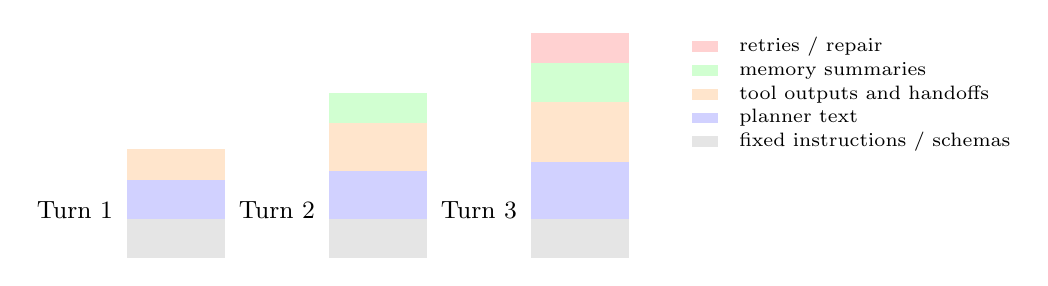
\begin{tikzpicture}[x=0.95cm,y=0.55cm]
  \node[font=\small] at (-0.7,1.1) {Turn 1};
  \node[font=\small] at (2.0,1.1) {Turn 2};
  \node[font=\small] at (4.7,1.1) {Turn 3};

  \fill[gray!20] (0,0) rectangle (1.3,0.9);
  \fill[blue!18] (0,0.9) rectangle (1.3,1.8);
  \fill[orange!20] (0,1.8) rectangle (1.3,2.5);

  \fill[gray!20] (2.7,0) rectangle (4.0,0.9);
  \fill[blue!18] (2.7,0.9) rectangle (4.0,2.0);
  \fill[orange!20] (2.7,2.0) rectangle (4.0,3.1);
  \fill[green!18] (2.7,3.1) rectangle (4.0,3.8);

  \fill[gray!20] (5.4,0) rectangle (6.7,0.9);
  \fill[blue!18] (5.4,0.9) rectangle (6.7,2.2);
  \fill[orange!20] (5.4,2.2) rectangle (6.7,3.6);
  \fill[green!18] (5.4,3.6) rectangle (6.7,4.5);
  \fill[red!18] (5.4,4.5) rectangle (6.7,5.2);

  \begin{scope}[shift={(7.55,4.75)}]
    \fill[red!18] (0,0) rectangle (0.35,0.25);
    \node[anchor=west, font=\scriptsize] at (0.5,0.125) {retries / repair};
    \fill[green!18] (0,-0.55) rectangle (0.35,-0.30);
    \node[anchor=west, font=\scriptsize] at (0.5,-0.425) {memory summaries};
    \fill[orange!20] (0,-1.10) rectangle (0.35,-0.85);
    \node[anchor=west, font=\scriptsize] at (0.5,-0.975) {tool outputs and handoffs};
    \fill[blue!18] (0,-1.65) rectangle (0.35,-1.40);
    \node[anchor=west, font=\scriptsize] at (0.5,-1.525) {planner text};
    \fill[gray!20] (0,-2.20) rectangle (0.35,-1.95);
    \node[anchor=west, font=\scriptsize] at (0.5,-2.075) {fixed instructions / schemas};
  \end{scope}
\end{tikzpicture}
\caption{Token accumulation across a trajectory. As an agent loops, fixed instructions remain, but planner text, tool outputs, summaries, and retries compound on top of them.}
\label{fig:token-stack}
\end{figure}

This is one reason agent orchestration is still brittle even when the base model is strong. $\tau$-bench and WebArena show that reliable task execution remains hard in realistic settings \cite{yen2024taubench,yao2023webarena}. Cuadron et al.\ show that overthinking in agentic tasks can raise cost sharply while hurting performance \cite{cuadron2025overthinking}. The practical lesson is that longer internal trajectories are not free, even when they sound more deliberative.

There is a second problem beyond raw token count: context position. Liu et al.\ show that long-context models often underuse information placed in the middle of a context window \cite{liu2024lostmiddle}. Agent systems make that failure mode worse because state that was highly relevant at step two may sit in the middle by step ten. Memory systems such as MemGPT attempt to manage that explicitly \cite{packer2023memgpt}, while benchmarks such as LoCoMo and LongMemEval show that long-horizon conversational memory remains brittle in practice \cite{maharana2024locomo,wu2024longmemeval}.

\begin{figure}[t]
\centering
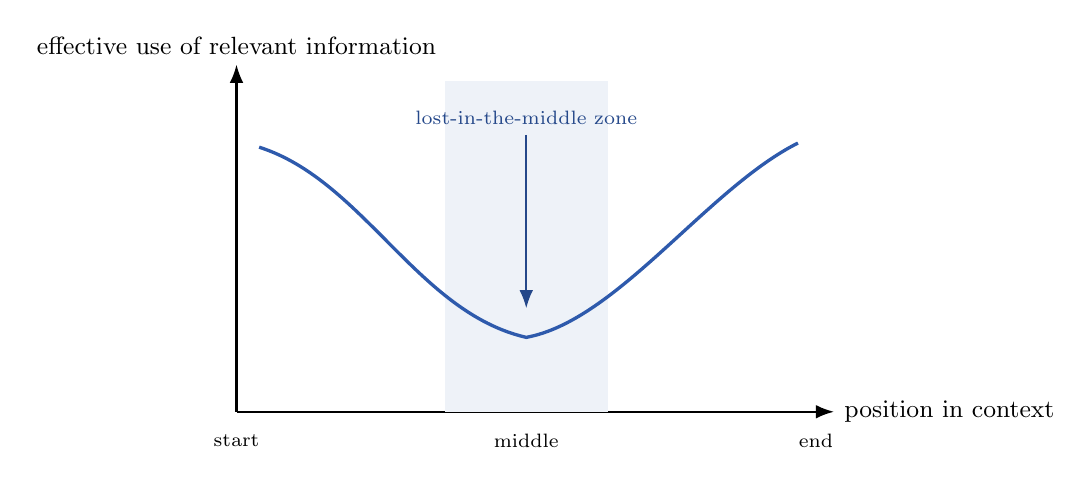
\begin{tikzpicture}[x=1.15cm,y=1.05cm]
  \draw[line] (0,0) -- (6.6,0) node[right, font=\small] {position in context};
  \draw[line] (0,0) -- (0,4.2) node[above, font=\small] {effective use of relevant information};
  \node[font=\scriptsize] at (0,-0.35) {start};
  \node[font=\scriptsize] at (3.2,-0.35) {middle};
  \node[font=\scriptsize] at (6.4,-0.35) {end};
  \fill[specblue!8] (2.3,0) rectangle (4.1,4.0);
  \draw[specblue, very thick] (0.25,3.2) .. controls (1.4,2.8) and (2.0,1.2) .. (3.2,0.9)
                                .. controls (4.2,1.1) and (5.2,2.7) .. (6.2,3.25);
  \node[font=\scriptsize, text=specblue!80!black] at (3.2,3.55) {lost-in-the-middle zone};
  \draw[specblue!80!black, thick, -Latex] (3.2,3.35) -- (3.2,1.25);
\end{tikzpicture}
\caption{Conceptual context-position failure. Agent trajectories often push earlier but still-relevant state into the middle of a growing prompt, where long-context models tend to use it less effectively.}
\label{fig:lost-middle}
\end{figure}

This is the systems backdrop for the present proposal. Language routing is interesting not because shorter languages are aesthetically appealing, but because orchestration already forces the system to choose what to keep, what to compress, and how to represent it.

\section{Research Questions and Hypotheses}

The first research question is whether internal Chinese, or a similarly compact language, reduces total billed tokens in realistic agent loops after fixed tool overhead is included. The second is where the benefit comes from: planner notes, memory updates, retry diagnoses, or inter-agent handoffs. The third is whether the gain is purely tokenization-driven or whether different internal languages elicit different reasoning paths. The fourth is whether a structured English protocol can match or beat free-form Chinese on schema-adjacent or code-heavy tasks. The fifth is whether a lightweight routing policy can outperform any single fixed language. The sixth is whether multilingual internal communication worsens prompt-injection risk, schema fidelity, or refusal behavior. The seventh is whether switching languages preserves semantic fidelity on terminology-heavy, culturally lexicalized, or domain-specific reasoning, or whether it introduces meaningful divergence even when end-task success appears unchanged.

\begin{figure}[t]
\centering
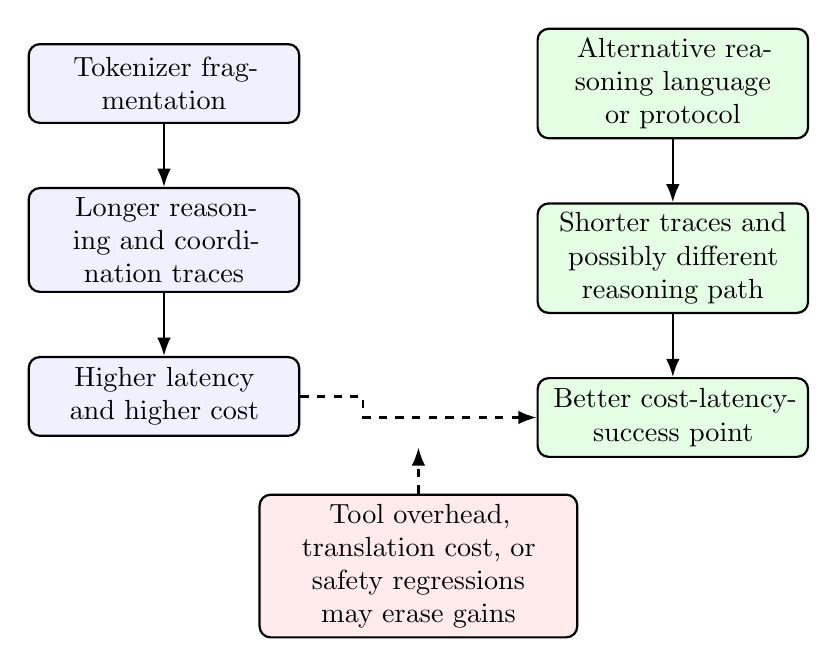
\begin{tikzpicture}[node distance=0.8cm and 1.0cm]
  \node[widebox, text width=3.2cm] (frag) {Tokenizer fragmentation};
  \node[widebox, text width=3.2cm, below=of frag] (long) {Longer reasoning and coordination traces};
  \node[widebox, text width=3.2cm, below=of long] (cost) {Higher latency and higher cost};
  \node[widebox, text width=3.2cm, right=3.0cm of frag, fill=green!10] (alt) {Alternative reasoning language or protocol};
  \node[widebox, text width=3.2cm, below=of alt, fill=green!10] (short) {Shorter traces and possibly different reasoning path};
  \node[widebox, text width=3.2cm, below=of short, fill=green!10] (pareto) {Better cost-latency-success point};
  \node[widebox, text width=3.8cm, below=1.1cm of $(cost)!0.5!(pareto)$, fill=red!8] (over) {Tool overhead, translation cost, or safety regressions may erase gains};
  \draw[line] (frag) -- (long);
  \draw[line] (long) -- (cost);
  \draw[line] (alt) -- (short);
  \draw[line] (short) -- (pareto);
  \draw[line, dashed] (cost.east) -- ++(0.8,0) |- (pareto.west);
  \draw[line, dashed] (over.north) -- ($(cost.south)!0.5!(pareto.south)$);
\end{tikzpicture}
\caption{Causal picture. The positive mechanism is plausible but not guaranteed; fixed overheads and safety costs may erase any free-text savings.}
\label{fig:causal}
\end{figure}

The main working hypothesis is that some internal agent messages behave like compression targets rather than user-facing prose. Planning, summarization, and memory updates are the likeliest candidates. The strongest competing hypothesis is that fixed tool prompts and schema-adjacent text dominate enough of the trajectory that language routing provides only cosmetic gains. A third possibility is that structured English or symbolic protocols, rather than any natural language, turn out to be the best compression medium. That is why the right baseline is not English-only. It is English plus strong compression and structured-reasoning baselines such as LLMLingua, Program-of-Thought, and symbolic chain-of-thought \cite{jiang2023llmlingua,pan2024llmlingua2,chen2022program,xu2024symbolic}.

\section{Experimental Program}

The experimental design should be paired and conservative. For each task family, the model, system prompt, tools, and seed band are held fixed while only the internal messaging policy changes. The comparison conditions are English-only, internal Chinese, controlled Chinese, English plus prompt compression, structured English, and a dynamic router that chooses among them. A Polish stress condition can be added as a deliberately inefficient contrast case rather than as a plausible deployment language.

\begin{figure}[t]
\centering
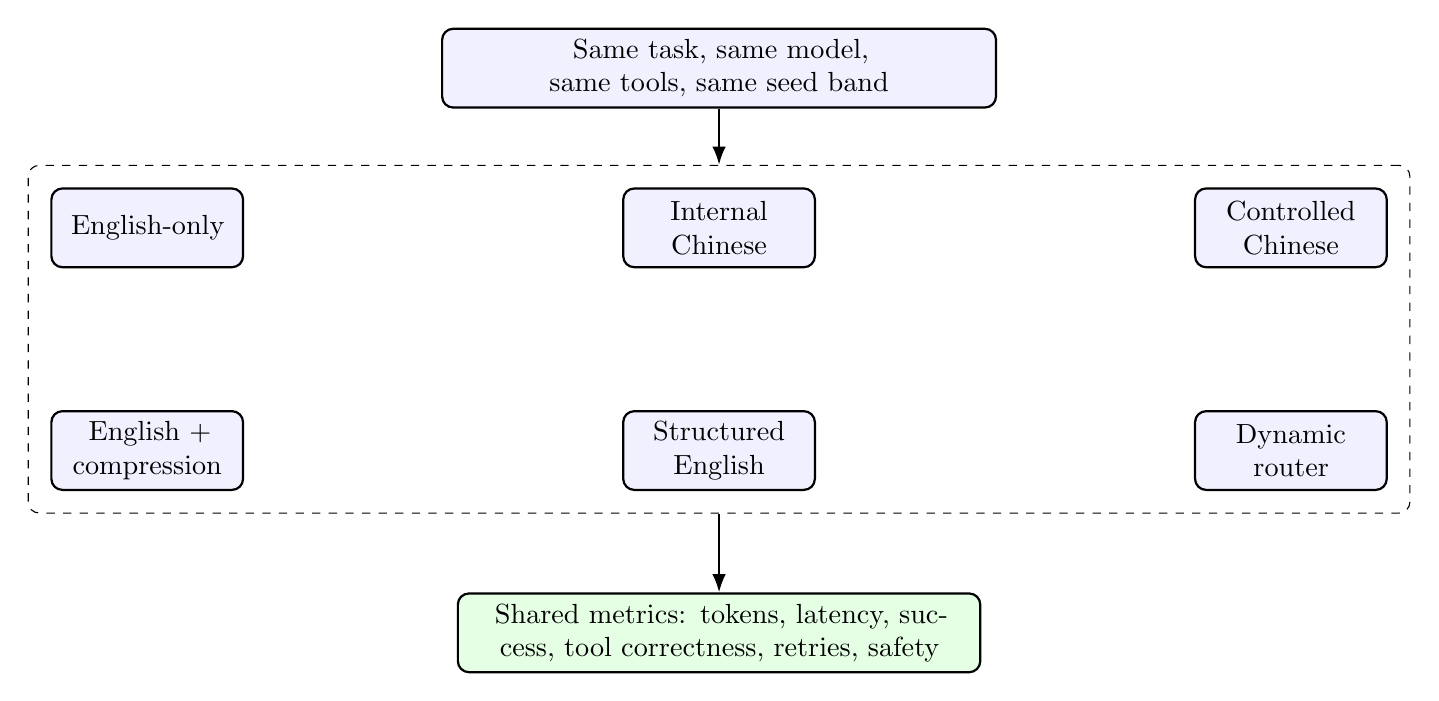
\begin{tikzpicture}[node distance=0.8cm and 0.6cm]
  \node[widebox, text width=6.8cm] (base) {Same task, same model, same tools, same seed band};
  \node[box, text width=2.2cm, below left=1.0cm and 2.5cm of base] (e1) {English-only};
  \node[box, text width=2.2cm, below=1.0cm of base] (e2) {Internal Chinese};
  \node[box, text width=2.2cm, below right=1.0cm and 2.5cm of base] (e3) {Controlled Chinese};
  \node[box, text width=2.2cm, below=1.8cm of e1] (e4) {English + compression};
  \node[box, text width=2.2cm, below=1.8cm of e2] (e5) {Structured English};
  \node[box, text width=2.2cm, below=1.8cm of e3] (e6) {Dynamic router};
  \node[draw, dashed, rounded corners=4pt, fit=(e1)(e2)(e3)(e4)(e5)(e6), inner sep=0.28cm] (group) {};
  \node[widebox, text width=6.4cm, below=1.0cm of group, fill=green!10] (metrics) {Shared metrics: tokens, latency, success, tool correctness, retries, safety};
  \draw[line] (base) -- (group);
  \draw[line] (group) -- (metrics);
\end{tikzpicture}
\caption{Evaluation design. Each condition is a policy over internal messages, not a change to final outputs or tool schemas.}
\label{fig:evaluation}
\end{figure}

The benchmark suite should emphasize realistic trajectories. WebArena is essential because it remains difficult enough that agent-side efficiency choices plausibly matter; its best GPT-4 baseline reaches only 14.41\% success versus 78.24\% human performance \cite{yao2023webarena}. X-WebAgentBench adds multilingual interactive web tasks \cite{wang2025xwebagentbench}. $\tau$-bench and API-Bank anchor the tool-use side, where argument correctness and policy compliance matter as much as answer quality \cite{yen2024taubench,li2023apibank}. SWE-bench can serve as an optional stress test for code-heavy messages, where named entities, paths, and stack traces likely reduce the value of internal translation \cite{jimenez2023swebench}.

The key metrics are total billed input tokens, total billed output tokens, wall-clock latency, task success, tool-call exact match, argument-level correctness, retry count, recovery success, and safety failure rate. The evaluation should also include semantic-fidelity checks on a targeted subset: entailment or consistency scoring between switched and unswitched traces, plus bilingual human review for terminology-heavy examples where token savings may hide loss of nuance. The most informative analysis is likely not a single scalar score but a Pareto frontier comparing cost and latency to task success and tool correctness, along with a message-level decomposition showing where savings arise. If all the gains come from planner notes while memory summaries and retry diagnoses degrade, that is still a useful scientific result.

\begin{figure}[t]
\centering
\begin{tikzpicture}[x=1.15cm,y=1.15cm]
  \draw[line] (0,0) -- (6.7,0) node[right, font=\small] {cost / latency};
  \draw[line] (0,0) -- (0,5.9) node[above, font=\small] {success / reliability};
  \filldraw[specgray] (5.4,3.5) circle (2.6pt);
  \filldraw[specblue] (4.4,4.25) rectangle +(0.11,0.11);
  \filldraw[specred] (4.95,4.75) -- ++(0.09,0.16) -- ++(0.09,-0.16) -- cycle;
  \node[draw=specgreen, fill=specgreen, diamond, minimum size=5.2pt, inner sep=0pt] at (2.9,5.05) {};
  \draw[specgreen, thick, dashed] (5.4,3.5) .. controls (4.9,3.95) and (4.0,4.8) .. (2.9,5.05);
  \begin{scope}[shift={(0.65,5.25)}]
    \filldraw[specgray] (0,0) circle (2.6pt);
    \node[anchor=west, font=\scriptsize] at (0.2,0) {English-only};
    \filldraw[specblue] (2.5,-0.055) rectangle +(0.11,0.11);
    \node[anchor=west, font=\scriptsize] at (2.75,0) {Internal Chinese};
    \filldraw[specred] (5.25,0) -- ++(0.09,0.16) -- ++(0.09,-0.16) -- cycle;
    \node[anchor=west, font=\scriptsize] at (5.55,0) {Compressed English};
    \node[draw=specgreen, fill=specgreen, diamond, minimum size=5.2pt, inner sep=0pt] at (0.0,-0.45) {};
    \node[anchor=west, font=\scriptsize] at (0.2,-0.45) {Dynamic router};
  \end{scope}
\end{tikzpicture}
\caption{Conceptual evaluation target. The project is successful if language routing moves the cost-latency-success frontier outward rather than merely reducing tokens in isolation.}
\label{fig:pareto}
\end{figure}

\section{Why A Routing Policy Is More Interesting Than A Single Language}

The best paper to write is probably not ``always use Chinese.'' Different internal message types have different failure modes. Code-adjacent messages are dense with file paths, stack traces, identifiers, and schema boundaries. Safety-critical instructions may be less tolerant of translation or compression. Planning notes and memory summaries, by contrast, may be almost ideal compression targets.

\begin{figure}[!htbp]
\centering
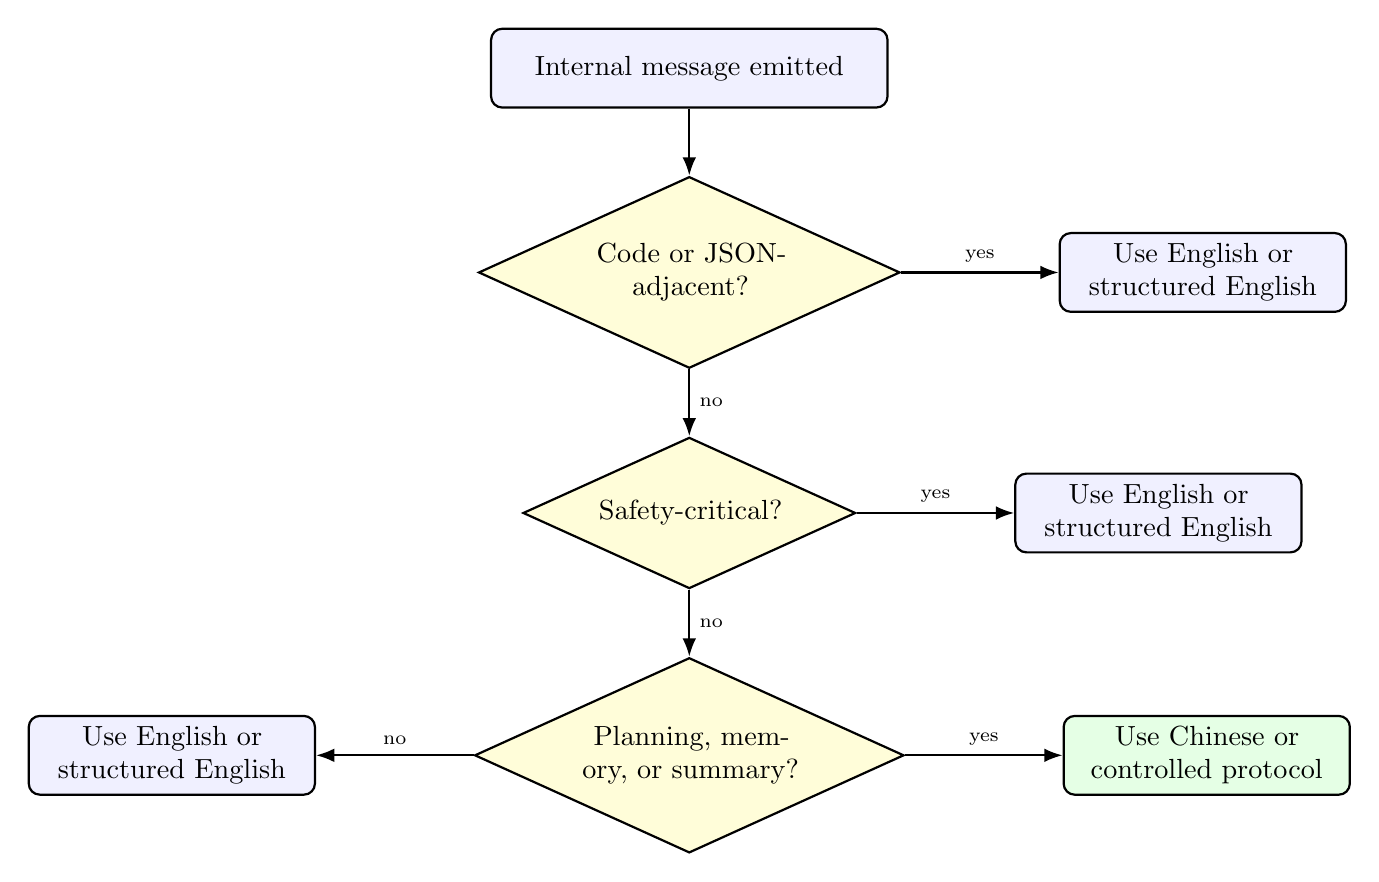
\begin{tikzpicture}[node distance=0.85cm]
  \node[box, text width=4.8cm] (start) {Internal message emitted};
  \node[decision, below=of start, text width=3.4cm] (code) {Code or JSON-adjacent?};
  \node[decision, below=of code, text width=3.2cm] (safe) {Safety-critical?};
  \node[decision, below=of safe, text width=3.5cm] (summary) {Planning, memory, or summary?};
  \node[box, text width=3.4cm, right=2.0cm of code] (eng1) {Use English or structured English};
  \node[box, text width=3.4cm, right=2.0cm of safe] (eng2) {Use English or structured English};
  \node[box, text width=3.4cm, right=2.0cm of summary, fill=green!10] (chi) {Use Chinese or controlled protocol};
  \node[box, text width=3.4cm, left=2.0cm of summary] (eng3) {Use English or structured English};
  \draw[line] (start) -- (code);
  \draw[line] (code.east) -- node[midway, above, font=\scriptsize] {yes} (eng1.west);
  \draw[line] (code) -- node[midway, right, font=\scriptsize] {no} (safe);
  \draw[line] (safe.east) -- node[midway, above, font=\scriptsize] {yes} (eng2.west);
  \draw[line] (safe) -- node[midway, right, font=\scriptsize] {no} (summary);
  \draw[line] (summary.east) -- node[midway, above, font=\scriptsize] {yes} (chi.west);
  \draw[line] (summary.west) -- node[midway, above, font=\scriptsize] {no} (eng3.east);
\end{tikzpicture}
\caption{Routing sketch. The high-value question is not which language wins globally but which message type prefers which internal protocol.}
\label{fig:router}
\end{figure}

This routing-policy framing has three advantages. First, it matches the actual structure of agent systems, which already distinguish planning, memory, and tool use. Second, it is scientifically stronger because it localizes the effect rather than globalizing it. Third, it creates a plausible negative-result regime: if only a narrow slice of messages benefits, the router will learn that and the paper can still report a useful boundary rather than a collapsed average.

\section{Risks, Safety, and Failure Modes}

The main risk is that the effect is real in single-turn reasoning but too small to matter in tool-heavy trajectories. Anthropic's current documentation warns that tool use introduces prompt overhead and that token accounting is model- and API-specific \cite{anthropic2026tokencount,anthropic2026tooluse}. If the variable free-text portion is small relative to fixed tool scaffolding, then language routing will matter only in planner-heavy tasks or long trajectories.

The second risk is safety. Song et al.\ show that multilingual blending can materially increase bypass rates relative to single-language inputs, with especially striking results on GPT-3.5 and GPT-4o \cite{song2025multilingual}. Wallace et al.\ argue more generally that instruction hierarchy matters because models often fail to distinguish privileged developer instructions from lower-trust text \cite{wallace2024instruction}. In an agent setting, tool outputs and retrieved documents are often semi-trusted at best. Any multilingual routing policy must therefore be evaluated not only for efficiency but also for injection resistance, refusal fidelity, and schema integrity.

\begin{figure}[!htbp]
\centering
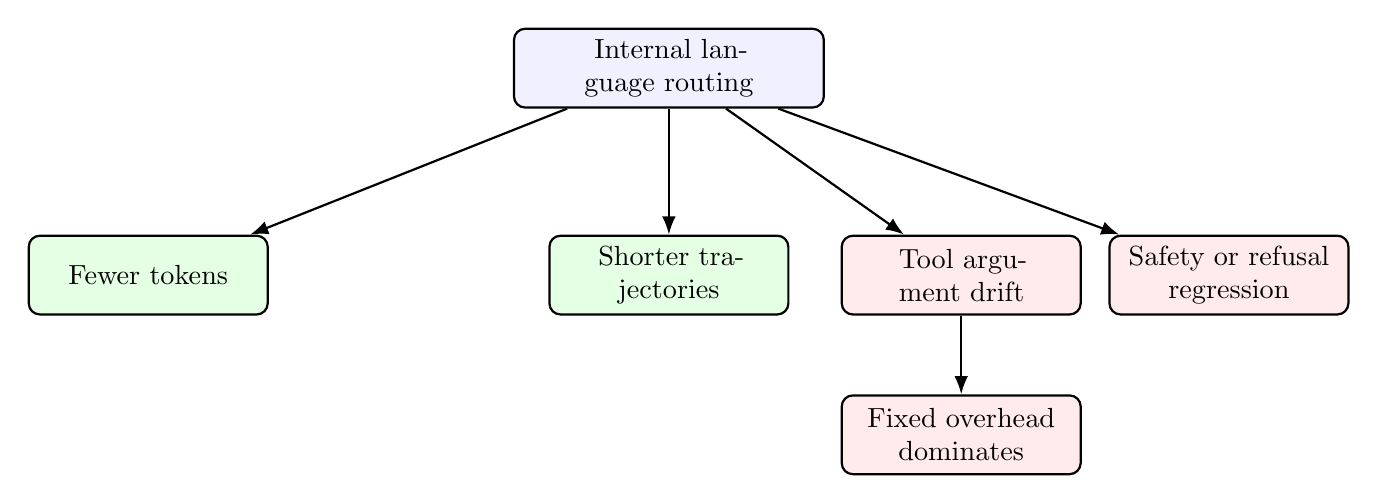
\begin{tikzpicture}[node distance=1cm and 0.95cm]
  \node[widebox] (root) {Internal language routing};
  \node[box, below left=1.6cm and 3.1cm of root, fill=green!10] (w1) {Fewer tokens};
  \node[box, below=1.6cm of root, fill=green!10] (w2) {Shorter trajectories};
  \node[box, below right=1.6cm and 0.2cm of root, fill=red!8] (r1) {Tool argument drift};
  \node[box, below right=1.6cm and 3.6cm of root, fill=red!8] (r2) {Safety or refusal regression};
  \node[box, below=of r1, fill=red!8] (r3) {Fixed overhead dominates};
  \draw[line] (root) -- (w1);
  \draw[line] (root) -- (w2);
  \draw[line] (root) -- (r1);
  \draw[line] (root) -- (r2);
  \draw[line] (r1) -- (r3);
\end{tikzpicture}
\caption{Failure surface. The same intervention can plausibly improve efficiency while degrading tool fidelity or safety if applied indiscriminately.}
\label{fig:failure}
\end{figure}

These risks are not reasons to avoid the project. They are precisely why the project is worth doing. If multilingual internal communication helps only on planner notes, that is still a useful systems result. If it helps nowhere once realistic overheads are counted, that is also a useful correction to an increasingly tempting intuition.

\section{Expected Contributions}

If successful, the project should deliver four things. First, it should provide a careful measurement study of when language routing changes the cost-latency-success frontier of agent trajectories. Second, it should provide a decomposition by message type, showing whether the gains arise in planning, memory, handoffs, retries, or nowhere. Third, it should compare natural-language routing against strong non-language baselines such as prompt compression and structured English protocols. Fourth, it should produce a lightweight routing policy that can be adopted or rejected on clear empirical grounds.

The novelty is therefore not multilingual prompting in isolation and not token compression in isolation. The novelty is to treat internal language choice as a systems policy over explicit agent message types and to evaluate that policy on realistic agent benchmarks with realistic safety constraints.

\section{Conclusion}

The project is timely because the necessary ingredients have only recently come together. Tokenization disparities are well documented. Reasoning models now expose mixed-language behavior that appears policy-relevant rather than accidental. Cross-lingual reasoning can reduce tokens without sacrificing accuracy. Agent benchmarks are strong enough that the effect can finally be tested in realistic multi-step settings. What remains genuinely open is whether internal language routing survives contact with tools, retries, memory, and safety.

The broader program now has a clearer shape as well. Language routing is the first paper because it is the cleanest inference-time variable to manipulate. Degradation detection is the trust layer that makes later claims defensible. Harness-vs-model is the meta-result that can justify the whole program. Abstract reasoning and monitorability sit further down the same spectrum of orchestration media, but they belong to the next phase once the language study is grounded.

\FloatBarrier
\begin{thebibliography}{99}

\bibitem{petrov2023unfairness}
Andrey Petrov, Emanuele La Malfa, Philip Torr, and Adel Bibi.
\newblock Language Model Tokenizers Introduce Unfairness Between Languages.
\newblock arXiv, 2023.
\newblock \url{https://arxiv.org/abs/2305.15425}.

\bibitem{limisiewicz2023tokenization}
Tomasz Limisiewicz, Jiri Balhar, and David Marecek.
\newblock Tokenization Impacts Multilingual Language Modeling: Assessing Vocabulary Allocation and Overlap Across Languages.
\newblock Findings of ACL, 2023.
\newblock \url{https://aclanthology.org/2023.findings-acl.350/}.

\bibitem{rust2023tokenizer}
Phillip Rust, Han Wang, et al.
\newblock Tokenizer Choice For LLM Training: Negligible or Crucial?
\newblock arXiv, 2023.
\newblock \url{https://arxiv.org/abs/2310.08754}.

\bibitem{einarsson2026scripttax}
Hakon Einarsson et al.
\newblock The Script Tax: Measuring Tokenization-Driven Efficiency and Latency Disparities in Multilingual Language Models.
\newblock arXiv, 2026.
\newblock \url{https://arxiv.org/abs/2602.11174}.

\bibitem{deepseek2025nature}
DeepSeek-AI et al.
\newblock DeepSeek-R1 Incentivizes Reasoning in LLMs through Reinforcement Learning.
\newblock Nature, 2025.
\newblock \url{https://www.nature.com/articles/s41586-025-09422-z}.

\bibitem{li2025bilingual}
Yihao Li, Jiayi Xin, Miranda Muqing Miao, Qi Long, and Lyle Ungar.
\newblock The Impact of Language Mixing on Bilingual LLM Reasoning.
\newblock EMNLP, 2025.
\newblock \url{https://aclanthology.org/2025.emnlp-main.1654/}.

\bibitem{wang2025mixing}
Mingyang Wang, Lukas Lange, Heike Adel, Yunpu Ma, Jannik Strotgen, and Hinrich Schutze.
\newblock Language Mixing in Reasoning Language Models: Patterns, Impact, and Internal Causes.
\newblock EMNLP, 2025.
\newblock \url{https://aclanthology.org/2025.emnlp-main.132/}.

\bibitem{ahuja2025efficientxlang}
Kabir Ahuja et al.
\newblock EfficientXLang: Towards Improving Token Efficiency Through Cross-Lingual Reasoning.
\newblock Findings of EMNLP, 2025.
\newblock \url{https://aclanthology.org/2025.findings-emnlp.845/}.

\bibitem{ramji2026abstractcot}
Keshav Ramji, Hamid Palangi, and Ramon Fernandez Astudillo.
\newblock Thinking Without Words: Efficient Latent Reasoning with Abstract Chain-of-Thought.
\newblock arXiv, 2026.
\newblock \url{https://arxiv.org/abs/2604.22709}.

\bibitem{schut2025english}
Lisa Schut, Yarin Gal, and Sebastian Farquhar.
\newblock Do Multilingual LLMs Think In English?
\newblock arXiv, 2025.
\newblock \url{https://arxiv.org/abs/2502.15603}.

\bibitem{tam2025languagematters}
Zhi Rui Tam, Cheng-Kuang Wu, Yu Ying Chiu, Chieh-Yen Lin, Yun-Nung Chen, and Hung-yi Lee.
\newblock Language Matters: How Do Multilingual Input and Reasoning Paths Affect Large Reasoning Models?
\newblock arXiv, 2025.
\newblock \url{https://arxiv.org/abs/2505.17407}.

\bibitem{qi2025yourlanguage}
Jirui Qi, Shan Chen, Zidi Xiong, Raquel Fernandez, Danielle Bitterman, and Arianna Bisazza.
\newblock When Models Reason in Your Language: Controlling Thinking Language Comes at the Cost of Accuracy.
\newblock Findings of EMNLP, 2025.
\newblock \url{https://aclanthology.org/2025.findings-emnlp.1103/}.

\bibitem{wang2023surveyagents}
Lei Wang, et al.
\newblock A Survey on Large Language Model based Autonomous Agents.
\newblock arXiv, 2023.
\newblock \url{https://arxiv.org/abs/2308.11432}.

\bibitem{yao2023react}
Shunyu Yao, Jeffrey Zhao, Dian Yu, Nan Du, Izhak Shafran, Karthik Narasimhan, and Yuan Cao.
\newblock ReAct: Synergizing Reasoning and Acting in Language Models.
\newblock ICLR, 2023.
\newblock \url{https://arxiv.org/abs/2210.03629}.

\bibitem{schick2023toolformer}
Timo Schick, et al.
\newblock Toolformer: Language Models Can Teach Themselves to Use Tools.
\newblock arXiv, 2023.
\newblock \url{https://arxiv.org/abs/2302.04761}.

\bibitem{wu2023autogen}
Qingyun Wu, et al.
\newblock AutoGen: Enabling Next-Gen LLM Applications via Multi-Agent Conversation.
\newblock arXiv, 2023.
\newblock \url{https://arxiv.org/abs/2308.08155}.

\bibitem{kim2023llmcompiler}
Yongchao Kim, et al.
\newblock An LLM Compiler for Parallel Function Calling.
\newblock arXiv, 2023.
\newblock \url{https://arxiv.org/abs/2312.04511}.

\bibitem{jiang2023llmlingua}
Huiqiang Jiang et al.
\newblock LLMLingua: Compressing Prompts for Accelerated Inference of Large Language Models.
\newblock EMNLP, 2023.
\newblock \url{https://aclanthology.org/2023.emnlp-main.825/}.

\bibitem{pan2024llmlingua2}
Zhuoshi Pan et al.
\newblock LLMLingua-2: Data Distillation for Efficient and Faithful Task-Agnostic Prompt Compression.
\newblock Findings of ACL, 2024.
\newblock \url{https://aclanthology.org/2024.findings-acl.57/}.

\bibitem{chen2022program}
Wenhua Chen et al.
\newblock Program of Thoughts Prompting: Disentangling Computation from Reasoning for Numerical Reasoning Tasks.
\newblock arXiv, 2022.
\newblock \url{https://arxiv.org/abs/2211.12588}.

\bibitem{xu2024symbolic}
Jundong Xu et al.
\newblock Faithful Logical Reasoning via Symbolic Chain-of-Thought.
\newblock ACL, 2024.
\newblock \url{https://aclanthology.org/2024.acl-long.720/}.

\bibitem{yao2023webarena}
Shunyu Yao et al.
\newblock WebArena: A Realistic Web Environment for Building Autonomous Agents.
\newblock arXiv, 2023.
\newblock \url{https://arxiv.org/abs/2307.13854}.

\bibitem{wang2025xwebagentbench}
Peng Wang, Ruihan Tao, Qiguang Chen, Mengkang Hu, and Libo Qin.
\newblock X-WebAgentBench: A Multilingual Interactive Web Benchmark for Evaluating Global Agentic System.
\newblock Findings of ACL, 2025.
\newblock \url{https://aclanthology.org/2025.findings-acl.988/}.

\bibitem{yen2024taubench}
Howard Yen et al.
\newblock $\tau$-bench: A Benchmark for Tool-Agent-User Interaction in Real-World Domains.
\newblock arXiv, 2024.
\newblock \url{https://arxiv.org/abs/2406.12045}.

\bibitem{li2023apibank}
Xiang Li et al.
\newblock API-Bank: A Comprehensive Benchmark for Tool-Augmented LLMs.
\newblock arXiv, 2023.
\newblock \url{https://arxiv.org/abs/2304.08244}.

\bibitem{jimenez2023swebench}
Carlos E. Jimenez et al.
\newblock SWE-bench: Can Language Models Resolve Real-World GitHub Issues?
\newblock arXiv, 2023.
\newblock \url{https://arxiv.org/abs/2310.06770}.

\bibitem{cuadron2025overthinking}
Andres Cuadron, et al.
\newblock The Danger of Overthinking: Examining the Reasoning-Action Dilemma in Agentic Tasks.
\newblock arXiv, 2025.
\newblock \url{https://arxiv.org/abs/2502.08235}.

\bibitem{liu2024lostmiddle}
Nelson F. Liu, Kevin Lin, John Hewitt, Ashwin Paranjape, Michele Bevilacqua, Fabio Petroni, and Percy Liang.
\newblock Lost in the Middle: How Language Models Use Long Contexts.
\newblock Transactions of the Association for Computational Linguistics, 2024.
\newblock \url{https://arxiv.org/abs/2307.03172}.

\bibitem{packer2023memgpt}
Charles Packer, Sarah Wooders, Kevin Lin, Vivian Fang, Shishir G. Patil, Ion Stoica, and Joseph E. Gonzalez.
\newblock MemGPT: Towards LLMs as Operating Systems.
\newblock arXiv, 2023.
\newblock \url{https://arxiv.org/abs/2310.08560}.

\bibitem{maharana2024locomo}
Adyasha Maharana, et al.
\newblock Evaluating Very Long-Term Conversational Memory of LLM Agents.
\newblock ACL, 2024.
\newblock \url{https://aclanthology.org/2024.acl-long.747/}.

\bibitem{wu2024longmemeval}
Dongming Wu, et al.
\newblock LongMemEval: Benchmarking Chat Assistants on Long-Term Interactive Memory.
\newblock arXiv, 2024.
\newblock \url{https://arxiv.org/abs/2410.10813}.

\bibitem{song2025multilingual}
Jiayang Song, Yuheng Huang, Zhehua Zhou, and Lei Ma.
\newblock Multilingual Blending: Large Language Model Safety Alignment Evaluation with Language Mixture.
\newblock Findings of NAACL, 2025.
\newblock \url{https://aclanthology.org/2025.findings-naacl.191/}.

\bibitem{wallace2024instruction}
Eric Wallace et al.
\newblock The Instruction Hierarchy: Training LLMs to Prioritize Privileged Instructions.
\newblock arXiv, 2024.
\newblock \url{https://arxiv.org/abs/2404.13208}.

\bibitem{baker2025monitoring}
Bowen Baker et al.
\newblock Monitoring Reasoning Models for Misbehavior.
\newblock arXiv, 2025.
\newblock \url{https://arxiv.org/abs/2503.11926}.

\bibitem{metr2025cotinformative}
METR.
\newblock CoT May Be Highly Informative Despite Unfaithfulness.
\newblock METR research note, 2025.
\newblock \url{https://metr.org/blog/2025-08-08-cot-may-be-highly-informative-despite-unfaithfulness/}.

\bibitem{anthropic2026tokencount}
Anthropic.
\newblock Token Counting.
\newblock Claude API Docs, accessed March 2026.
\newblock \url{https://docs.anthropic.com/en/docs/build-with-claude/token-counting}.

\bibitem{anthropic2026tooluse}
Anthropic.
\newblock Tool Use with Claude.
\newblock Claude API Docs, accessed March 2026.
\newblock \url{https://docs.anthropic.com/en/docs/agents-and-tools/tool-use/overview}.

\end{thebibliography}

\end{document}
